% Overleaf compiler: pdfLaTeX
\documentclass[sigconf,anonymous,review,balance=false]{acmart}

\usepackage{booktabs}
\usepackage{graphicx}
\usepackage{microtype}
\usepackage{subcaption}

\title{RealRF-DG: Source-Aware Dual-Domain Learning for Data-Efficient
Radio Fingerprinting Across Real Capture Environments}

\author{Anonymous Author(s)}
\affiliation{\institution{Anonymous Institution}}

\begin{abstract}
Radio-frequency fingerprinting models are frequently evaluated on generated
signals or a single capture setup, making it difficult to distinguish device
features from dataset shortcuts. We present RealRF-DG, a reproducible
multi-source benchmark and dual-domain model trained on deterministic 10\%
subsets of three real-signal corpora. The model fuses temporal raw-I/Q features
with spectral magnitude and phase-step features, uses source-specific device
heads, and applies gradient-reversal regularization to reduce source leakage.
All dataset selections, splits, hardware tuning decisions, and predictions are
exported as auditable artifacts.
\end{abstract}

\begin{document}
\begin{CCSXML}
<ccs2012>
 <concept>
  <concept_id>10010147.10010257.10010293.10010294</concept_id>
  <concept_desc>Computing methodologies~Neural networks</concept_desc>
  <concept_significance>500</concept_significance>
 </concept>
</ccs2012>
\end{CCSXML}
\ccsdesc[500]{Computing methodologies~Neural networks}
\keywords{radio-frequency fingerprinting, domain generalization, deep
learning, real signals, physical-layer authentication}
\maketitle

\section{Introduction}
State the practical authentication problem, the risk of generated-signal
benchmarks, and the paper contributions.

\section{Related Work}
Cover RF fingerprinting, cross-domain robustness, complex-signal neural
networks, and data-efficient learning.

\section{Datasets and Protocol}
We use only publisher-released real captures from WIDEFT, INRIA PLA, and the
WLAN environment corpus~\cite{siddik2021wideft,alla2026pla,stojke2026wlan}.
\begin{figure*}[t]
  \centering
  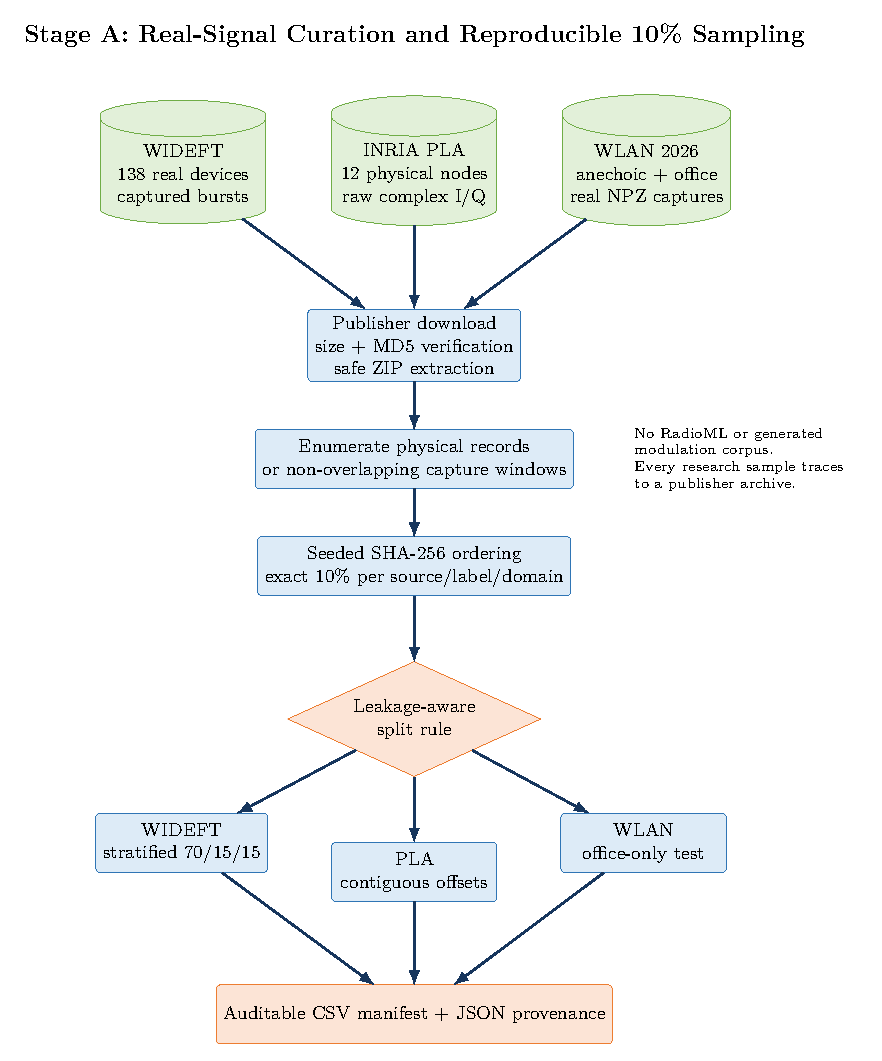
\includegraphics[width=0.92\textwidth,page=1]{methodology_diagrams.pdf}
  \caption{Checksum-verified real-data curation and deterministic 10\% sampling.}
  \label{fig:data}
  \Description{Flowchart from three real RF datasets through checksum
  verification, deterministic ten-percent selection, leakage-aware splits,
  and an auditable manifest.}
\end{figure*}

\section{Method}
\begin{figure*}[t]
  \centering
  \includegraphics[width=0.92\textwidth,page=2]{methodology_diagrams.pdf}
  \caption{Dual-domain source-aware RF fingerprinting architecture.}
  \label{fig:model}
  \Description{Parallel temporal and spectral branches feed a Transformer and
  shared embedding with source-specific classification, supervised
  contrastive, and gradient-reversal objectives.}
\end{figure*}

\section{Experimental Setup}
Report all hyperparameters, the measured L4 batch size, software versions,
three random seeds, and the ablation plan.

\section{Results}
\begin{table}[t]
  \centering
  \caption{Replace placeholders only with completed experiment results.}
  \begin{tabular}{lccc}
    \toprule
    Source & Accuracy & Macro F1 & ECE \\
    \midrule
    WIDEFT & -- & -- & -- \\
    INRIA PLA & -- & -- & -- \\
    WLAN office holdout & -- & -- & -- \\
    \bottomrule
  \end{tabular}
\end{table}

\section{Limitations and Ethics}
Discuss receiver/channel confounding, the 10\% compute constraint, lawful use,
device tracking risks, and limits on generalization.

\section{Conclusion}
Summarize findings without overstating deployment readiness.

\bibliographystyle{ACM-Reference-Format}
\bibliography{references}
\end{document}
